\chapter{OpenCog AGI框架}{The OpenCog Artificial General Intelligence Architecture}

在本章我们将介绍通用人工智能体系结构OpenCog的一些关键技术。OpenCog是一个由多个子系统组成的庞大智能认知体系结构。更多有关此系统的技术,可以参考这本一千多页的书籍【XX】。在此我们只列出与本文研究紧密联系的几个关键的子系统,这样有助于理解本文的研究内容,包括前文中提到的自然语言理解、自然语言生成、逻辑推理以及智能会话系统建模等。
\section{ConPrime设计}{The CogPrime Design}

\indent OpenCog框架的核心是一个认知概念框架,称为CogPrime,但它们两者并不完全等同。OpenCog是一个更泛化的框架,用来实现许多特定AI程序以及可能的AGI设计。同时CogPrime可以单独被实现,而不要求被置于OpenCog框架中。一个在OpenCog中特别实现的CogPrime版本被称为OpenCogPrime。OpenCog是作为CogPrime的一个高效的、规划化的实现来设计的。

本节将概述CogPrime,它是一个实现AGI的概念和技术的框架,以一系列理论为基础。CogPrime的具体实现和测试(在OpenCog框架之内)仍然处在一个较浅的阶段,CogPrime的目标是表现出与人类智力性质接近的泛化智能,并最终可以被扩展到更广泛的领域的智能功能(?)。

CogPrime将在《Engineering General Intelligence》一书中有更详尽的描述[??],它将有超过1000页的篇幅,包括附录。本文的目标是以更紧凑的形式列举出其中一些关键点。在此我们略去CopPrime与其他已有的认知框架的比较,读者可以阅读以下文章[??],其中介绍了当前人工大脑与AGI构架的发展形式,其中包含了一个与较早版本的CogPrime框架的比较。

\subsection{认知协同:CogPrime的核心设计概念}{Cognitive Synergy: A Central Design Concept in OpenCog}
\indent CogPrime核心概念基础是以下三点:
\begin{itemize}
  \item 智能取决于系统的整体知识库中的特定高级结构和动力学的涌现;
  \item 我们尚未发现任何可以涌现出这类结构的算法或方案;
  \item 试图通过在一个系统内整合若干个不同的AI算法和框架来实现这种涌现的过程是微妙的,这些算法与框架的整合方式需要仔细地注意,而到目前为止这种整合并没有以正确的方式被执行。
\end{itemize}

人脑表现为许多不同的结构与动力学的整合,以通用的组件按照可感知的认知结构来组合到一起。然而,大脑的算法和结构被进化过程所影响,各部分紧密地联系在一起,互相适应,就像身体的不同器官之间的互相适应一样。这种协作使得整个系统表现出人类水平的泛化智能。我们相信,目前的AI中所缺少的部分是认知协同:不同组件的互相适应形成了整体恰当上的认知架构,在这个过程中,组件间以动态的方式充分地互相协作、彼此间紧密地相互联系在一起,就像人脑和身体的各部分一样,使得整体的架构和动力学涌现出来。这让我们得到CogPrime的核心假设之一:在一个恰当的认知框架和环境中,通过整合多重的符号和亚符号的学习和记忆组件,可以产生出与人类相当甚至更强的稳定的智能。

这类紧密的整合之所以尚未被充分探索,是因为它涉及到不同的层次,需要进行困难的框架和组件算法设计,这种设计应该保有某种面向架构和动力学的视角,使得它处在一个创造了合适的环境的系统中,以显现出架构和动力学。典型的,与不同的认知功能相对应的AI算法和架构已经通过各个研究者社区基于不同的理论规则进行了部署,并针对每个具体的运行环境进行的相应的性能调校。让这些性能迥异的组件共同工作在一起,并形成真正的协作是难以完成的任务。我们相信,以现有技术创造人类等级的AGI的“关键调料”,正是这种协同,而非一些特定的算法、结构、或架构原则。

\subsection{目前的和将来优先的OpenCog应用}{Current and Prior Applications of OpenCog}
为了更好地理解,到目前用来实现CogPrime的具体平台,我们将简略地讨论通过OpenCog系统实现CogPrime架构的部分工作。

OpenCog是一个开源的软件框架,以CogPrime架构的“OpenCogPrime”实现为目标(目前只是部分实现),已被用于自然语言处理和数据挖掘的商业应用。例如,参考[?]中OpenCogPrime的PLN推理以及RelEx语言处理被整合到一起,用来自动化地处理基于从PubMed中收集的信息的生物假设生成(?biological hypothesis generation)。[?]描述了使用OpenCog的MOSES组件进行生物信息分析;它的用途还被延伸到一些未被公开发表的商业应用中,例如财务预测、基因组、市场营销数据分析以及自然语言处理。在最近的相关工作中,OpenCog被用来控制虚拟世界中的虚拟代理[?]。
在2007-2008年间完成的原型工作涉及到使用一个叫OpenPetBrain的OpenCog的变形来控制虚拟世界中的狗。这些OpenCog控制的虚拟狗并没有表现出接近现实中狗的(或人类小孩)的智力,但它们展示了一系列有趣的相关功能,包括:
\begin{itemize}
  \item 基于模仿和强化来学习新的行为;
  \item 响应自然语言的命令和问题,作出恰当的行为和自然语言的回答;
  \item 自发地探索它们的世界,利用记忆来调整未来的学习和语言交互;
\end{itemize}

受游戏“我的世界”的启发,目前OpenCog正在将对虚拟狗的控制工作扩展到使用OpenCog控制游戏中的虚拟主体。这些主体最初被特别设定了各自在游戏世界中要达成的目标,为了完成这些目标,他们需要通过搬运“砖块”和使用简单的英语交流。这些任务可以是:

\begin{itemize}
\item 学习建造台阶或梯子来拿到高处的物体;
\item 学习建造掩体来躲避入侵者;
\item 学习建造环境中存在的类似结构物体
\item 学习建造桥梁以跨越峡谷。
\end{itemize}

当然,这一类任务中AI的显著性取决于系统能给予什么样的反馈、以及环境的复杂程度。让AI以非常独特的方式去做这些事情会相对简单,但这并非项目的主旨——目标是让系统通过涉身的经验以及少量的人类教师的反馈,学会使用泛化学习机制和泛化认知框架去完成类似任务。如果能成功,这将为今后的AGI研发提供一个非常不错的平台,就像一个可视化的和(immediately meaningful?)OpenCog的demo。

本文在写作时,项目团队的注意力集中在一些特定的任务上,包括:
\begin{itemize}
\item 观察另一主体通过建筑来到达高处的过程
\item 我们发现让虚拟主体观察另一个主体在一个不同的语境中,通过建造来到达高处的步骤,并模仿他的行为是一个不错的办法
\item 同时,如果虚拟主体需要一个特定的高处的物体,但是周围没有建造台阶所需的材料,那么尝试通过其他办法来达到高处(包括比如建造梯子或者让一个个子高的主体去帮他拿)
\item 我们发现,如果该主体需要隐藏自己有价值的物品,避免比自己更大的生物拿走它,那么他需要建造一个带有小洞的容器,这样该主体可以躲进去,但是比它大的生物无法进入。
\end{itemize}

延伸该工作到虚拟主体中,在2009-2010年间,预实验已经通过OpenCog在Nao机器人上进行过了[?]。这些涉及到将OpenCog与一个分离的控制底层感知和行动的子系统的整合。这个整合仅通过相当简单的方式进行,然而,如何进行该整合是论文[?]和[?]中讨论的话题,本文仅仅介绍到此。在此方面的工作在2013-2015年间一直在进行中,由Hong Kong Innovation in Technology Fund的一个基金赞助。

\subsection{概念背景}{Conceptual Background}
\indent CogPrime的设计研发受到一种叫“模式主义”的心灵哲学影响[?]。模式主义心灵哲学是对如何实现智能系统的统筹思考。它基于一个简单的前提,即心灵由模式组成——同时心灵是一个对它自己和世界的模式识别系统,尤其是那些关于在何种语境下、何种过程会导致何种结果的模式。然而,CogPrime受模式主义视角的指引这一点不应被过分解读。CogPrime是一个集成设计,通过若干不同的哲学、科学以及工程的想法的结合来形成,它的成功或失败并不取决于某一特定的哲学对智能的理解。

在细节上,追寻模式主义哲学会导致一系列特定的关于心灵本质的假设和结论。通过智能在复杂环境中完成复杂行为,我们发现一个认知系统的动力学会被一下两种因素影响:
\begin{itemize}
\item 自组织,通过系统动力学引起退出系统的模式来产生一个新的(???);
\item 面向目标的行为,在[?]中有严格的定义,但基本上相当于一个与环境交互的系统,该系统的行为类似于求某些可理解的简单函数的最大值。
\end{itemize}

自组织和面向目标行为应该被理解为互相协作的两个方面。举一个详细的例子,一个虚拟主体被要求通过一些砖块建造一个惊人的建筑,这是面向目标的。但是该主体如果在之前有过在自法的、无结构性的玩耍砖块的过程,那么它能更好地完成该面向目标的任务。同时这种要求它建造一个惊人的砖块结构的“创造力的推动”可能引起它去探索,以得到一些新奇的模式,而它可能将这些模式重新用于将来的非结构性的砖块游戏中。

基于以上概念,如[?]中所讨论的,我们可以假定若干主要的动力学原则,包括:
\begin{itemize}
\item 演化,作为一个主要过程,通过它,可以在很大数量的模式中挑选出一些,用于形成新模式的基础,基于一些与主体所要完成的任务相关的“适应度函数”;
\item 自生成:该过程让拥有多个模式交互的系统维持它的整体性,当系统中的一个模式开始降低其强度(?Intensity)时,一些其他的模式会增加他们的强度,以使得该遇到麻烦的模式重新开始增加它的强度;
\item 联系,给予注意力的模式,会将注意力散布一部分在其他曾经有过联系模式上。同时,根据皮尔斯的心灵定律[?],简述之,即心灵是一个互相联系的记忆网络,它的机制是,记忆中的每一个想法都是一个激活的智能体(agent),这个网络持续地与那些和它有关联的记忆发生作用 ;
\item 差别的注意力分配;评分系统。那些被评价为对达成目标更有价值的模式会被给予更多的注意力,并被鼓励参与新模式的生成;
\item 模式创造,被井架为对实现目标更有价值的的模式被变异与组合来产生新的模式。
\end{itemize}

接下来,按照[?]中列出的许多理由,我们假定智能系统中的模式网络必然引起一下大规模产生的结构
\begin{itemize}
\item 层次化网络。模式被与控制其他代表了更特化方面的模式所联系起来。
\item heterarchical网络(?)。系统维持一个关于那些曾经与其他模式相联系的模式的记忆。
\item 双网络。这两种结构被合并,通过一种机制让它们和谐共处。通过许多可能的方式,层次化地组织起一批模式,并保证层次结构中接近的模式有更多通向彼此的有意义的heterarchical连接;当然,必须有一个在层次结构中接近的模式间搜索heterarchical连接的机制。
\item 自结构。网络中模式的一部分形成了整个网络的结构的大致的图景。
\end{itemize}

CogPrime并没非直接由这些哲学规则产生;它最初通过合并人类认知心理学和计算机科学算法结构而创建,然后修改这个组合以产生一个系统,使它看起来与这些哲学规则相一致的、并且以当前的硬件基础在计算上可行,它还将包括一个大致上与人类相似的认知结构。CogPrime的成功将主要取决于这些高阶结构和机制是否能够通过CogPrime中表达和算法的系统交互中产生出来,它们将被用于在恰当的环境中控制恰当的主体。在[?]中详细讨论了这些抽象的概念如何从CogPrime的结构和算法中具体地产生出来。

\subsection{CogPrime的高阶架构}{High-Level Architecture of OpenCog}

图\ref{fig:CogPrime1}描述了CogPrime的高阶架构。一个关键的潜在原则是:与多种类型的记忆相联系的多认知过程的运用,将会使得一个智能主体执行它认为在当前环境下对完成目标最有利的过程。例如,在机器人学龄前阶段的条件下,最高层的目标将会是日常的事物,如取悦老师、学习新的知识和技能、保护机器人的身体。

将这些图表与人类的认知结构图表进行对比是有趣的\cite{Goertzel2012a},它将概述目前所理解的人类认知结构。二者主要的区别在于,CogPrime的图表用于特定的结构(如知识表征)和过程,然而泛化的整合性图表架构仅仅只涉及结构和过程。举例来说,整合图表涉及陈述性知识和学习,然而CogPrime图表指的是PLN,一个关于陈述性知识的推理和学习的特定系统。在\cite{Goertzel2010a}中用一个表格来表示CogPrime图表和以整合图表表示的人类认知结构、过程之间的联系,这表示了被每个CogPrime组件所实例化泛化的认知功能。

\begin{figure*}[htb]
\centering
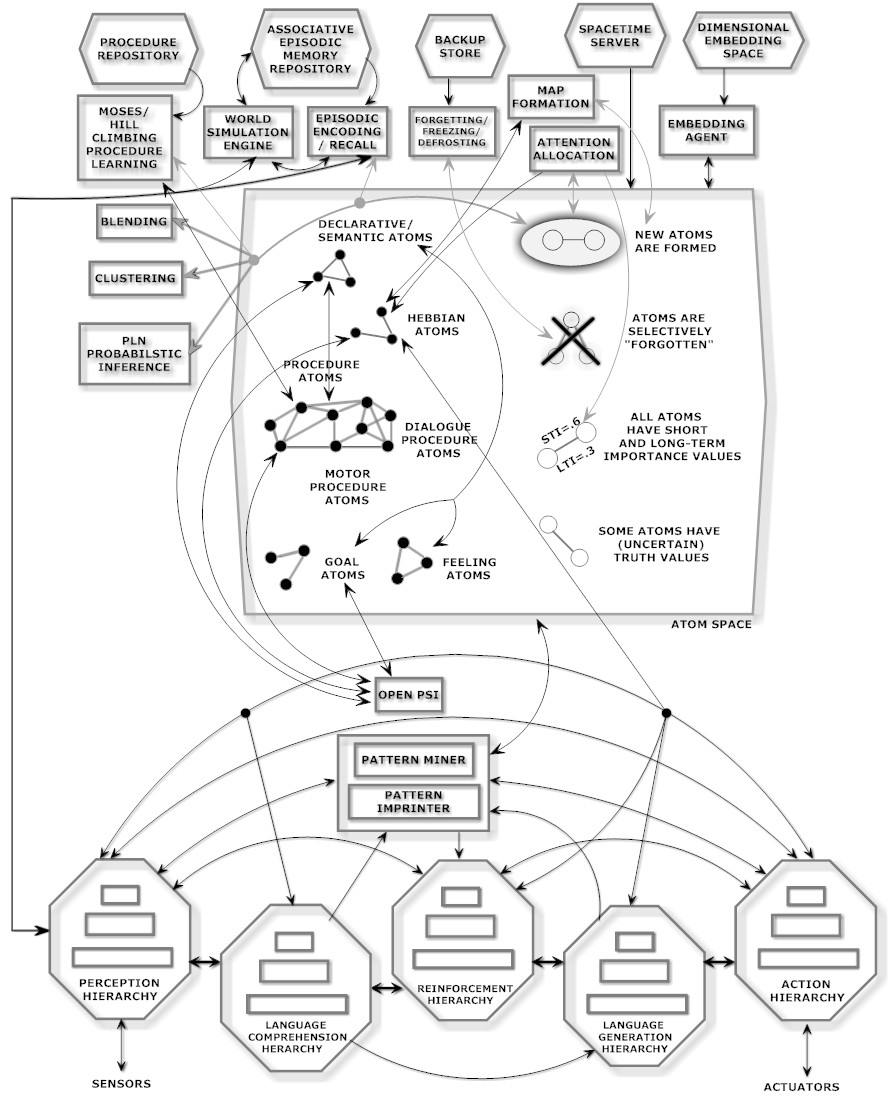
\includegraphics[width=14cm]{figures/1.jpg}
\caption{ {\bf High-Level Architecture of OpenCog.}  This is a conceptual depiction, not a detailed flowchart (which would be too complex for a single image).   }
\label{fig:CogPrime1}
\end{figure*}

\subsection{表征和记忆}{Representation and Memory}

\paragraph{本地和全局知识表征}

OpenCog的知识表征机制在根本上是基于{\it 网络}的。把精神当作网络的观点是隐含在模式主义哲学中的,因为每一个模式都可以被看成某物的模式,或关于某物的布置的模式——因而一个模式总是可以被看做二个或更多物体之间的关系。一系列的模式形成一个模式网络。各类知识可以以网络形式来表达,而认知过程也可以被表达为网络,举例来说将它们表达为程序,以各种树或图的形式表达。在一个智能中模式的涌现可以 被看作自身的一个模式网络;在涉身的心灵和它的物理和社会环境之间的关系可以被看做某种生态和社会网络。

知识表达系统的两个主要超类是{\it 局部}(也被称为{\it 显示})和全局(也被称为{\it 隐式})系统,我们用一个被称为{\it 全局-局部}的混合类包含了这两者。在一个{\it 局部}系统中,每一条知识都是用一小部分认知系统的元素来存储的;在一个{\it 全局}系统中,每一条知识都被以一种特定的模式存储与激活,比如以认知系统的一定比例的元素的形式;在一个{\it 全局-局部}混合系统中,这两种方式被共同使用。以上三种知识表征类型都可以被网络所实现。在CogPrime中,这三者都是以{\it 同样}的网络(Atomspace)来实现。

\paragraph{CogPrime中的记忆类型和相关认知处理}

CogPrime依靠多种的记忆类型,如同上面所讨论的,它的前提是正确地建立一个类人AGI系统,以处理不同类型的记忆,这些记忆包括了结构和动力学。

CogPrime的记忆类型有:陈述性记忆、过程性记忆、感知记忆、以及场景记忆,这些在认知科学中被广泛讨论\cite{Tulving2005}的记忆类型,以及分配泛用的系统资源的注意力记忆、和为特定目标分配系统资源的意向性记忆。表格\ref{tab:opencog}概述了这些记忆类型,给出了关键的引用并指出了相关的认知过程,同时指出了每一个认知过程(模式创造、联系等)所对应的泛化的模式主义认知动力学。

以模式主义认知理论的形式,CogPrime中的多种记忆类型可被看做特定类型模式的特化存储方式,并经过了计算时间与空间上的优化。联系到某种特定类型的记忆的认知过程被用来创造和识别该记忆的类型。原则上所有类型的模式都可以在统一的记忆和处理构架下进行,CogPrime所用到的这种类型特例化,是为了能够在现有的计算条件可接受的前提下创造有效的泛化智能。我们在\cite{Goertzel2010c}中所详细论述过,高效性并不是可有可无的,而是对真实世界中的泛化智能举足轻重的特性(就像Hutter所展示的,如果没有效率的限制,任意登记的泛化智能都可以通过简单而琐碎的程序来实现)。

CogPrime设计的本质在于,与每种类型的记忆相关的数据结构和处理过程是被紧密联系在一起的,相比于仅仅包含同一种结构和处理过程的而仅仅以不同的黑盒分割开的构架,它产生了协同性的智能。

OpenCog中设计有交互的认知处理过程,以使得不同类型的记忆间可以互相转换,尽管有时这会消费较多的计算资源(比如,一段陈述性的知识可能通过一些努力被解释为过程性或场景性的知识);同时,对于一个主要处理某一种类型记忆的学习进程来说,它可能会经常通过把知识转换成其他类型来解决问题,比如认知协同任务。

\newcolumntype{Y}[1]{>{\centering\hspace{0pt}\arraybackslash}m{#1}}

\begin{table*}[ht]
\centering
\begin{tabular}{|Y{3cm}|Y{5cm}|Y{3cm}|}
\hline \textbf{记忆类型} & \textbf{特定的认知过程} & {\bf 泛化的认知功能} \\ \hline
\textbf{陈述性} & 概率逻辑网络PLN\cite{Goertzel2008}; 概念调整\cite{Fauconnier2002} & 模式创造 \\ \hline
\textbf{过程性} & MOSES(一个创新的概率演化运算学习算法)\cite{Looks2006} & 模式创造 \\ \hline
\textbf{场景性} & 内部模拟引擎\cite{Goertzel2008d} & 联系,模式创造 \\ \hline
\textbf{注意性} & 经济注意力网络(ECAN)\cite{Goertzel2010} & 联系,评分 \\ \hline
\textbf{意向性} & 概率目标层次按照OpenPsi动机框架通过PLN和ECAN来细化\cite{Bach2009}) & 评分,模式创造 \\ \hline
\textbf{感知} & 在CogBot中通过DeSTIN组件来支持 & 联系,注意力分配,模式创造,评分 \\ \hline
\end{tabular}%
\caption{CogPrime中的记忆类型和认知处理过程。第三列表示每一个特定的认知处理过程所拥有的泛化认知功能,它们给予认知的模式主义理论.}
\label{tab:opencog} 
\end{table*}

%%%%%%%%%%%%%%%%%%%%%%%%%%%%%%%%%%%%%%%%%%%%%%%%%%%%%%%%%%%%%%%
\section{OpenCog中AtomSpace的表示形式}{OpenCog AtomSpace Representation}
\label{sec:atoms}
%%%%%%%%%%%%%%%%%%%%%%%%%%%%%%%%%%%%%%%%%%%%%%%%%%%%%%%%%%%%%%%

XXXX备用:其基本的存储单元称为“原子”(Atom)。每一个Atom携带的值(Value)的结
构为(STI,LTI,TruthValue,Confidence,Content)。STI(Short Term Importance)
和LTI(Long Term Importance)可以用来模拟短期记忆(Short Term Memory)和长期
记忆(Long Term Memory)。XXXX

正如上述所言,Atomspace是OpenCog中所使用统一且通用的知识库,它使用包含特定类型的节点(Node)和链接(Link)的加权有向超图结构来表示知识,主要用作表示叙述性的知识,同时亦间接地表示其它类型的知识。这些特定类型的节点和链接是经过包括语义层面的细心挑选,以满足OpenCog在认知过程的需要。由于OpenCog的Atomspace表示形式是本文的核心,在这里我们会详细列出几个简单的示例予以说明。

以下是一个以OpenCog常用的表示方法去表示OpenCog中的链接的例子:
 
{\tt\begin{small}\begin{lstlisting}
InheritanceLink Lian_Ruiting animal <.99>
\end{lstlisting}\end{small}}

\noindent 或更明确地:

 {\tt\begin{small}\begin{lstlisting}
InheritanceLink <.99>
	ConceptNode "Lian_Ruiting"
	ConceptNode "animal "
\end{lstlisting}\end{small}}

以及:

{\tt\begin{small}\begin{lstlisting}
EvaluationLink <.7>
	chase 
	ListLink
		cat
		mouse
\end{lstlisting}\end{small}}

\noindent 或更明确地:

{\tt\begin{small}\begin{lstlisting}
EvaluationLink <.7>
	PredicateNode "chase" 
	ListLink
		ConceptNode "cat"
		ConceptNode "mouse"
\end{lstlisting}\end{small}}

\noindent 正如上述示例所示,节点通常具有名称,而链接则没有,但链接可以连接一个或多个的目标,而这些目标可以是节点或链接。

综合来说,Atomspace是一个“带标记的通用超图“,这些标记可以是节点的名称或其真值等等。“超图“与一般“图“的其中一个主要不同之处在于其链接,例如ListLink或SetLink,它是可以连结两个以上的参数,而其通用性也允许这些链接与其他的链接相连,而不只局限于节点。

另一个值得注意的地方是这些节点的名称,虽然在这些示例中它们都是以英语来表示,但实际上OpenCog会在日常操作中透过自主学习去创造一些新的节点,而这些节点往往都不会和我们的语言概念相对应。

更重要的一点是, AtomSpace的知识表示形式的主要功能是提供一个灵活的方式去紧凑地表达多种相关形式的知识,并允许它们之间有交互操作。其中的“交互操作“是指,例如,一组的陈述性的知识可以跟另一组的注意力相关或程序性相关的知识相互连结,或一组在一个类别的知识可以跟另一组在其他类别的知识重叠在一起(同一链接同时有著一个陈述性相关的真值和一个注意力相关的重要值)。总而言之,只要有任何表示形式能够提供足够的灵活性来:

\begin{itemize}
\item 紧凑地表达所有在人类记忆中扮演著主导角色关键类别
\item 灵活地创建特定的副表示形式去表达在上述这些关键类别中的知识,同时又能够被迅速地改动或操纵这些知识
\item 重叠和连结不同种类的知识,包括上述这些特定的副表示形式
\end{itemize}

\noindent 以上几项都符合OpenCog的整体要求。而这些Atom的表示形式已能满足此计设的总体要求,并从软件的角度来看已证明是可行的。

\subsection{基本的Atom种类}{Basic Atom Types}

在OpenCog中最基本而且经常会用到的Atom种类中的节点是:

\begin{itemize}
\item ConceptNode -- 表达任何的单元,具体或抽象但又不能以其他特定的节点种类来表达的概念
\item PredicateNode  -- 表达一个为Atom产生真值的程序(以下会有详细说明)
\item SchemaNode -- 表达一个以一个Atom产生另一个Atom的程序,或产生一些其他效果
\end{itemize}

和以下的链接:

\begin{itemize}
\item MemberLink -- 连结一个通用种类的Atom和一个ConceptNode,并拥有一个模糊真值
\item InheritanceLink -- 连结两个ConceptNodes,并拥有一个概率真值
\item SimilarityLink -- 连结两个ConceptNodes,并拥有一个概率真值
\item EvaluationLink -- 连结一个PredicateNode以及其参数
\item ExecutionLink -- 连结一个SchemaNode、其需要的参数以及其产生的输出
\begin{itemize}
\item ExecutionOutputLink -- 连结一个SchemaNode以及其输入,当遇到特定的认知程序时才会产生输出
\end{itemize}
\end{itemize}


\subsection{绑定程序的节点}{Grounded Procedure Nodes}

SchemaNode和PredicateNode有两种形态:已绑定和未绑定。未绑定是指系统尚未知道应该如何评定该方案,或系统将会以一连串的ExecutionOutputLinks来绑定该方案。而已绑定的会有一个特定程序的名称(目前该程序可以是C++,Scheme或Python语言编写的程序)来执行该方案。例如:

\begin{verbatim}
ExecutionOutputLink
	GroundedSchemaNode "plus.py"
	ListLink
		NumberNode "2"
		NumberNode "3"
\end{verbatim}

\noindent 当执行时,会调用Python函数“plus“来把“2“和“3“加起来,然后产生一个名为“5“的NumberNode作为其输出。

\subsection{內涵与外延的关系}{Intensional and Extensional Relationships}


OpenCog的链接类型中亦有多种拥有继承和相似性质的链接,例如IntensionalInheritanceLink和ExtensionalInheritanceLink,其细节将会在\cite{PLN}中详述,但简而言之,以下链接的真值:

\begin{verbatim}
ExtensionalInheritanceLink A B
\end{verbatim}

\noindent 同时亦可被表示为:

\begin{verbatim}
SubsetLink A B
\end{verbatim}

\noindent 是一个条件概率$P(B|A)$。另一方面,以下链接的真值:

\begin{verbatim}
ExtensionalInheritanceLink A B
\end{verbatim}

\noindent 是一个条件概率$P(prop(B)|prop(A))$,当中$prop(X)$表示在PLN推理系统中定义的模糊集合X的属性。

\subsection{SatisfyingSet}{SatisfyingSet}
SatisfyingSet的算符能够表达一个集合关系的概念,而当中每一位成员都是乎合同一个述语的元素,并用Member的关係形式,以一个模糊数值(而非概率数值)来表达该元素属于一个概念的真确性。

举例来说,假设现在有“FriendOfBob“这个述语和三个元素“Jack“、“John“和“Jill“:

\begin{verbatim}
Evaluation <.7>
	FriendOfBob
	Jack

Evaluation <.6>
	FriendOfBob
	John

Evaluation <.8>
	FriendOfBob
	Jill
\end{verbatim}

根据SatisfyingSet算符的定义,我们会得出以下的Member:

\begin{verbatim}
Member <.7>
	Jack
	SatisfyingSet
		FriendOfBob

Member <.6>
	John
	SatisfyingSet
		FriendOfBob

Member <.8>
	Jill
	SatisfyingSet
		FriendOfBob
\end{verbatim}

\subsection{等效式与启示式}{Equivalence and Implication}

现在我们可以为述语定义等效式与启示式,如同为概念定义相似式和继承式一样:

\begin{verbatim}
Equivalence
        A
        B
\end{verbatim}

是等同于:

\begin{verbatim}
Similarity
        SatisfyingSet(A)
        SatisfyingSet(B)
\end{verbatim}

以及:

\begin{verbatim}
Implication
        A
        B
\end{verbatim}

是等同于:

\begin{verbatim}
Inheritance
        SatisfyingSet(A)
        SatisfyingSet(B)
\end{verbatim}

以上是混合了等效式与启示式的表达形式。内涵与外延的表达形式都是以类似的方式去表达,以下是一个ExtensionalEquivalence的例子:

\begin{verbatim}
ExtensionalEquivalence
        A
        B
\end{verbatim}

是等同于:

\begin{verbatim}
ExtensionalSimilarity
        SatisfyingSet(A)
        SatisfyingSet(B)
\end{verbatim}

\subsection{Boolean链接}{Boolean Links}

Boolean链接是用来表达一些常用操作的概率:ANDLink、OrLink、NOTLink和XORLink。

同时,就像其他编程语言般,Atomspace亦有“IfElseLink“以作为一个判断选择的条件简写:

\begin{verbatim}
ElseLink
	R
		A
		B
	C
\end{verbatim}

是等同于:

\begin{verbatim}
AND
	R
		A
		B
	R
		NotLink
			A
		C
\end{verbatim}

\noindent 这个设计能有效防止产生过多的链接种类,例如IfImplicationElse、IfExtensionalImplicationElse、IfIntensionalImplicationElse、IfInheritanceElse等等。
	
		
\subsection{真值}{Truth Values}
\label{真值}

一个Atom的真值是用来表示一个Atom的\textit{真确性},在某程度上是取决于Atom的类型。这个数值是以一个TruthValue物件的形式跟Atom链接在一起。一般来说我们会在Atom的表示式后以\ensuremath{<}\ensuremath{>}及一个数字来显示其真值,例如:

\begin{verbatim}
A <.4>
\end{verbatim}

來表示一個名稱为“A“的Atom的真值为.4。同样地:

\begin{verbatim}
IntensionalInheritanceLink Ben monster <.5,.9>
\end{verbatim}

\noindent 来表示一个连接著“Ben“和“monster“的IntensionalInheritance关係中有著一个.5的强度和.9确信情度。总而言之,\ensuremath{<}tv\ensuremath{>}表示著一个平均值为tv的概率分佈。这些概念和语义将会在\cite{PLN}中作详细展述。

\subsection{量词}{Quantifiers}  

在不明确逻辑理论中,量化过程是一个比较细微的事项。PLN包含了标準的ForAll和ThereExists的量词(使用高阶概率定义的概率真值),在处理量化过程时主要会用AverageQuantifier来建构,例如:

\begin{verbatim}
AverageQuantifier $X
        F($X)
\end{verbatim}

的真值为F(\$X)的真值的加权平均值,即是以下的总和:

\begin{verbatim}
w($X) F($X) / N
\end{verbatim}

\subsection{总结——语言相关的Atom类型}{Summary of Language-Relevant Atom Types}

接下来将会描述一些用来表达具体语言概念的Atom类型。

原则上,要处理从ASCII编译的语言资料,除了需要CogPrime结构外就只有以下两个节点类型和一个链接类型:

\begin{itemize}
\item CharacterNode
\item CharacterInstanceNode
\item ListLink
\end{itemize}

\noindent 因而字串就可以以列表或拼接的方式来表达,例如“pig“可以以列表$(\#p, \#i, \#g)$来表达。

然而,实际上定义特定的語言Atom类型也很有帮助的,例如:

\begin{itemize}
\item	MorphemeNode/ MorphemeInstanceNode
\item		WordNode/WordInstanceNode
\item		PhraseNode/PhraseInstanceNode
\item		SentenceNode/ SentenceInstanceNode
\item		UtteranceNode/ UtteranceInstanceNode
\end{itemize}





\subsection{基于类型理论的Atomspace形式化表示}{A Formal Type System for OpenCog’s Atomspace}

引入Atomspace的形式化表示能容许我们在不用关注输入是否完全正确的情况下精密地应用Atomspace,并能在某些情况下减少制造混乱的同时又提高系统的精确度。为实现这目的,我们建立了一个基于类型理论的形式化表示机制,具体来说,我们采用了Haskell的泛代数数据类型 \cite{Haskell2014}对Atomspace形式化如下:

\begin{verbatim}
data TV = SimpleTV Float Float

data ConceptName = ConceptName String

data VariableName = VariableName String

data Atom a where
	-- TV
	TV :: TV -> Atom TV
	TVAnd :: Atom TV -> Atom TV -> Atom TV
	TVOr :: Atom TV -> Atom TV -> Atom TV
	TVGetTV :: Atom a -> Atom TV

	-- Predicate
	Predicate :: (Atom a -> TV) -> Atom (Atom a -> TV)
	PredicateAnd :: (a ~ (Atom b -> TV)) => Atom a -> Atom a -> Atom a
	PredicateOr :: (a ~ (Atom b -> TV)) => Atom a -> Atom a -> Atom a
	Implication :: (a ~ (Atom b -> TV)) => Atom a -> Atom a -> Atom TV
	Equivalence :: (a ~ (Atom b -> TV)) => Atom a -> Atom a -> Atom TV
	Evaluation :: (Atom (Atom a -> TV)) -> Atom a -> Atom TV

	-- Concept
	Concept :: ConceptName -> Atom ConceptName
	ConceptAnd :: Atom ConceptName -> Atom ConceptName -> Atom ConceptName
	ConceptOr :: Atom ConceptName -> Atom ConceptName -> Atom ConceptName
	Inheritance :: Atom ConceptName -> Atom ConceptName -> Atom TV
	Similarity :: Atom ConceptName -> Atom ConceptName -> Atom TV
	Member :: Atom a -> Atom ConceptName -> Atom TV
	SatisfyingSet :: Atom (Atom a -> TV) -> Atom ConceptName
	
	-- Variable
	PredicateVariable :: VariableName -> Atom (Atom a -> TV)
	ConceptVariable :: VariableName -> Atom ConceptName
	TVVariable :: VariableName -> Atom TV
	Variable :: VariableName -> Atom a

	-- Binding
	Bind :: Atom a -> Atom TV -> Atom (Atom a -> TV)

	-- Quantifier
	ForAll :: Atom a -> Atom TV -> Atom TV
	Exists :: Atom a -> Atom TV -> Atom TV

	-- number
	Number :: (Num a) => a -> Atom a

	-- Schema
	Schema :: (a ~ (Atom b -> Atom c)) => a -> Atom a
	ExecutionOutput :: (a ~ (Atom b -> Atom c)) => Atom a -> Atom b -> Atom c

	-- List
	List :: [Atom a] -> Atom [Atom a]
\end{verbatim}	

以下是一些使用该形式化机制表示Atomspace超图的例子:

\begin{verbatim}
-- Functions from Atom to TV to build predicates
is_bottom :: Atom a -> TV
is_bottom = undefined
is_top :: Atom a -> TV
is_top = undefined
is_car :: Atom a -> TV
is_car = undefined

-- And/Or hypergraph of concepts
a = Concept (ConceptName "A")
b = Concept (ConceptName "B")
c = Concept (ConceptName "C")
h1 = ConceptOr (ConceptAnd a b) c

-- And/Or hypergraph of predicates
h2 = PredicateOr (PredicateAnd (Predicate is_top) (Predicate is_car)) (Predicate is_bottom)

-- Apply Evaluation to predicate h2
tv3 = Evaluation h2 (List [Concept (ConceptName "BMW")])

-- Build a Schema
add :: (Atom [Atom Float]) -> Atom Float
add (List [Number x, Number y]) = Number (x + y)
add _ = undefined
h4 = Schema add -- :: Atom (Atom [Atom Float] -> Atom Float)

-- Apply a Schema
h5 = ExecutionOutput h4 (List [Number 3, Number 4]) -- h5 :: Atom Float

-- Test GetTVLink
tv1 = TVGetTV h1
tv2 = TVGetTV h2

-- Test AndLink with TV
tv4 = TVAnd tv1 tv3
\end{verbatim}	

%%%%%%%%%%%%%%%%%%%%%%%%%%%%%%%%%%%%%%%%%%%%%%%%%%%%%%%%%%%%%%%
\section{OpenCog的模式匹配器Patter Matcher}{The OpenCog Pattern Matcher}
%%%%%%%%%%%%%%%%%%%%%%%%%%%%%%%%%%%%%%%%%%%%%%%%%%%%%%%%%%%%%%%

其中一个在OpenCog语言处理中最常使用的工具是一个模式匹配器。OpenCog的模式匹配器是一个查询引擎或变数配对者,主要功用是在Atomspace中寻找特定的模式,或是一些Atom相关排列或“模板“。在轮入一个等定的Atom排列(即一个超图)后,模式匹配器会从Atomspace中寻找所有合乎条件的超图。同时一些“空白位置“,即“变数“在一个超图的位置,亦可存在于该输入的超图当中,而模式匹配器则会“填补“这些“空白位置“。例如:“John threw a \_\_\_\_).“亦可以被判断为“John threw a ball.“,前提是在查询前该句子要存在于Atomspace里,而在这个例子中“ball“就是被配对的一个答案。输入的超图中可以在不同的地方拥有多过一个的“空白位置“,同时亦可以有多过一个的答案。在这过程中,BindLink提供了一个便利的API去达到这目的,接下来会有更多的技术层面说明。

模式匹配器是一个变数配对者,是在传统计算机科学中“统一“的概念,因为这是它的功能之一。它同时亦是一个查询引擎,因为这个变数配对过程某情度上是等同于用SQL在关联数据库中进行查询。当中主要的分别在于在OpenCog中概念是以超图的形式表示,所以它亦可以被形容为一个超图查询语言HQL(Hypergraph Query Language)。但这些都只是以不同的名称去表示同一个程序。

这个模式匹配器亦是结构精密应用的一个重要组件,同时亦是建立前向和后向链接的一个重要基础。它拥有C++和Scheme的接口以供不同的应用。

模式匹配器是由数个不同的组件连接在一起,组成一个基础前向链接或超图重写的工具。在其核心是一个能比较和配对不同超图以及其变数的组件,而这个组件跟另一个“找寻器“一同使用便能寻找整个Atomspace中的合乎条件的超图。最后一个组件是一个“编写器“,主要功用是当有一个配对成功产生后建立一个或以上在ImplicationLink后半部列明的超图。

这个模式匹配器接受有指定“规则“的BindLinks,再把这些“规则“应用到Atomspace里。每一个“规则“是一个ImplicationLink,以“if P then Q“的形式表达,当中P和Q分别代表不同的超图。如果P被实现了,那么便能得到Q。Q可以是任何种类的超图,但如果Q是一个ExecutionLink,这便意味著当P被实现了,系统便将会实行其他程序,这在整体来说可以是一个十分强大的功能,因为在一般情况下很多程序都可以以ExecutionLink来执行。

模式匹配器不会更改任何超图中的真值(Truth Value)或关注值(Attention Value),有需要时使用者亦可以自行编写和执行相关的程序。

在默认的回调函数中模式匹配器会搜索整个Atomspace,因此亦有需要编写特定的回调函数以限制其搜索范围,例如只寻找和接受拥有某程度短期重要性的Atom,以只获取相对重要的资讯。

以下是一个使用模式匹配器的示例:

\begin{verbatim}
(define find-animals
  (BindLink
    ;; The variable to be bound
    (VariableNode "$var")
    (ImplicationLink
      ;; The pattern to be searched for
      (InheritanceLink
         (VariableNode "$var")
         (ConceptNode "animal")
      )
 
      ;; The value to be returned.
      (VariableNode "$var")
    )
  )
)
 \end{verbatim}
 
只要在OpenCog Scheme shell中输入以下指令便能执行以上的模式匹配器以找出在Atomspace中所有继承“animal“的概念:

\begin{verbatim}
(cog-bind find-animals)
\end{verbatim}


%%%%%%%%%%%%%%%%%%%%%%%%%%%%%%%%%%%%%%%%%%%%%%%%%%%%%%%%%%%%%%%
\section{概率逻辑网络PLN}{Probabilistic Logic Networks}
\label{sec:pln}
%%%%%%%%%%%%%%%%%%%%%%%%%%%%%%%%%%%%%%%%%%%%%%%%%%%%%%%%%%%%%%%

概率逻辑网络PLN是OpenCog的一个很特殊的方面,在此文中它讲被重点提出,尤其在第\ref{chap:inference}章,PLN是一个独特的推理系统,它嵌入了预测逻辑和传统逻辑的组合。PLN在\cite{Goertzel2008, RWR}中被详细介绍。在此我们给出一个高阶的概述。

PLN是一个数学和软件框架,用于非确定推理、操作CogPrime软件框架、使概率真值与泛化逻辑推理规则的整合成为可能。具体来说,PLN包含:

\begin{itemize}
\item 一系列推理规则(例如,演绎、贝叶斯规则、变量归一化、演绎推理,等等),每一项都有一个或多个逻辑关系或词项(以CogPrime的原子来表征)作为输入,并计算输出;
\item 特定的数学方程,基于合适的背景前提假设的概率值,计算结论的概率值。
\end{itemize}
PLN还涉及一条特殊的功能,评估概率值的置信度(证据的分量,或二阶的不确定性)。最后,PLN在软件中的实现需要重要的抉择,要求考虑推理规则的结构化表征、“推理控制”——这种策略要求,在每个特定的实际情况中,判断以何种顺序做何种推理。

\subsection{PLN的一个简单概述}{A Simple Overview of PLN}

PLN的关键因素是它的规则和方程式。总的来说,一个PLN规则有:

\begin{itemize}
\item 输入:一个原子元组(它必须满足某些要求,视规则而定)
\item 输出:一个原子元组
\end{itemize}

实际上,几乎在所有情况下,输出都是一个单一的原子,而输入则是一个单一的原子或者是一对原子。

特定的原形例子是演绎规则,它的输入是这样的:

{\tt\begin{small}\begin{lstlisting}
X_Link A B
X_Link B C
\end{lstlisting}\end{small}}

而它的输出应该是这样的:

{\tt\begin{small}\begin{lstlisting}
X_Link A C
\end{lstlisting}\end{small}}

在这里,X\_Link可以是继承性链接、子集链接、按时链接或延伸按时链接的。

一个PLN方程与一条PLN规则同时存在,它表示了输出的非确定性真值,基于输入的非确定真值。例如,如果我们有:

{\tt\begin{small}\begin{lstlisting}
X_Link A B <sAB>
X_Link B C <sBC>
\end{lstlisting}\end{small}}



那么标准的PLN演绎方程告诉我们

{\tt\begin{small}\begin{lstlisting}
X_Link A C <sAC>
\end{lstlisting}\end{small}}

其中: 

$$
s_{AC}=s_{AB}s_{BC}+\frac{\left(1-s_{AB}\right)\left(s_C-s_Bs_{BC}\right)}{1-s_B}
$$, $s_A$表示节点$A$的真值强度。

在这个例子中,每一个院子的非确定真值通过一个“强度”数值来给出。总的来说,PLN中的非确定真值可以有多种形式,比如:

\begin{itemize}
\item 单一的强度值,比如0.8,这表示概率或模糊真值,取决于具体的原子类型
\item (强度,置信度)对,比如(0.8,0.4)
\item (强度,数量)对,如(0.8,15)
\item 非确定的概率值,如(0.6,0.9, 0.95),这表示概率间的相互评分
\end{itemize}

\subsection{前向和后向链}{Forward and Backward Chaining}

PLN中典型的模式的使用是前向链和后向链推理。

前向链表示:

\begin{enumerate}
\item 给出一个感兴趣的原子池(列表);
\item 应用PLN规则到这些原子上,以产生新的原子,最好也是感兴趣的;
\item 将这些新的原子加如到池中,返回步骤1。
\end{enumerate}

例子:“人是动物”和“动物会吸”是两个池中的原子。它们被演绎规则所组合,形成了结论“人会呼吸”

后向链分为两种情况,第一种:

\begin{itemize}
\item “真值查询”,给出一个原子目标,它的真值未知(或者过于不确定),以及一个原子池,按照演绎规则,通过组合池中原子,找到一种方法来评估该目标原子的真值。
\end{itemize}

例子:目标是“人是否会呼吸?”(继承链接“人会呼吸”)。目标的真值通过“人是动物,动物会呼吸,因此人会呼吸”的推理来评估。

第二种:

\begin{itemize}
\item “填空查询”,给定一个目标链接(原子可以是节点或链接)以及一个或多个目标中间的变量原子,找出什么原子可以被放在变量原子的位置上,可以使目标链接获得一个高的置信度(即一个“高的真值”)。
\end{itemize}

例子:目标是“什么会呼吸”,即“继承链接\$X呼吸”……直接在原子空间中查找发现院子“继承链接 动物会呼吸”,表示空格\$X的位置上可以被填入“动物”。推理揭示“继承链接 人会呼吸”,因此空格\$X也可以被填入“人”。

例子:目标是“什么会呼吸和加法”,即“(继承链接\$X会呼吸)并且(继承链接\$X会加法)”。推理揭示此处\$X可以被填入“人”但不能是“猫”或“电脑”。

常识推理可能涉及一个前向和后向链的组合。

推理中最困难的部分是“推理控制”——在可能的推理步骤中选取哪些步骤,以获得需求的信息(在后向推理中)或获得感兴趣的新信息(在前向推理中)。在一个有大量原子的原子空间中有许多可能的和强大的启发信息需要进行选择。推理控制的最佳指导是某些基于系统的过去推理历史的归纳。当然,一个较信的系统不会有很多的历史信息。依靠非直接的相关历史是一个推理问题——这个问题的最好解决是让系统有一些历史经验。

\subsection{一阶概率逻辑网络}{First Order Probabilistic Logic Networks}

我们以更正式的方式来介绍PLN。PLN被氛围一阶和高阶子理论(FOPLN和HOPLN)。这些词项源自NARS\cite{Wang2006}。我们首先使用了FOPLN,然后他们使用了HOPLN。

FOPLN是一个传统逻辑,设计到词项(term?)和词项间的关系(链接)。它是一个非确定逻辑,词项和关系都拥有真值对象,真值对象有多种可能的类型,从单一的数值到复合的结构如非确定概率。词项可以是基本的观察,或一个符号集合$T$中的抽象的符号。

